% !TeX spellcheck = en_US
\section{Models for the Recording Position}
\label{sec:440_recording_position}
The results describe the distance to a recorded event, classified by the shot type and the angle under which it was recorded.
\subsection{Impact of the Distance}
The impact of the distance to the \ac{AoI} is important for the perceived quality. 
Figure~\ref{fig:440_Distance_Music} shows the distribution of the perceived quality for varying distances using a constant angle. 
It indicates that the distance has an observable effect for different recordings.
\begin{figure}
\centering
 \subfloat[Music - Concert]{  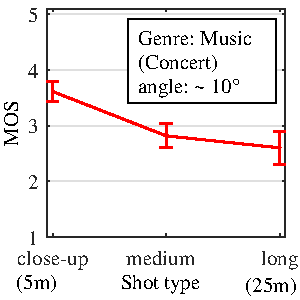
\includegraphics{./gfx/400_UGV_Quality/Distance_Music.pdf}}
 \subfloat[Scenery - Eiffel tower]{   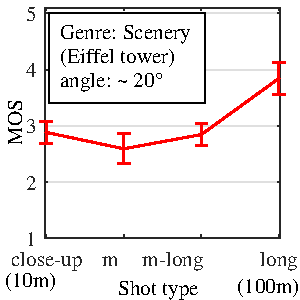
\includegraphics{./gfx/400_UGV_Quality/Distance_Scenery.pdf}}
  \subfloat[Sports - Motorbike]{  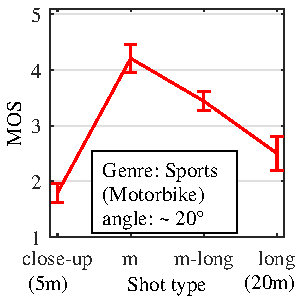
\includegraphics{./gfx/400_UGV_Quality/Distance_Sports2.pdf}}
\caption[Perceived quality of recordings from different recording distances]{Perceived quality of recordings from different distances with the same orientation for (a) Music, (b) Scenery and (c) Sports.}
\label{fig:440_Distance_Music}
\end{figure}
For the "show" and "music" genre, results indicate that the close-ups are seen as the preferred shot type for short music recordings.
A close-up represents a recording showing the main performer, e.g., in the concert recording. 
The quality difference between the close-up to the other shot types is small (see Figure \ref{fig:440_Distance_Music} a) and nearly indistinguishable. 
Distances ranging from 5 up to 30 meters are preferred in all "show" and "music" sequences. 
Distances beyond 30 meters lead to a significant drop in the perceived quality due to the frame size of the videos and the technical limitations of smartphone camera sensors (genre: "music").

Also, the workers are asked to annotate the \ac{RoI}. 
In most cases, it shows a larger region of the scene, but the subregion capturing the close-up is preferred in music clips.
A more significant drop of the perceived quality is observed for the sequences in the genres "scenery" as well as "sports". 
In the case of the scenery sequences, e.g., the video sequence "Scenery 1" (see Figure \ref{fig:440_Distance_Music} b), the perceived quality increases with increasing distance, as in the long shot, the complete \ac{RoI} can be seen.
"Scenery" recordings include a wider border region around the \ac{RoI} in comparison to the other sequences, which indicates that the viewers are more interested in the surroundings of the \ac{PoI}. 
For the "sports" recordings, medium shots showed the main actor, e.g., the soccer player leading the ball, or the motorbike rider performing stunts.
This distance is preferred in comparison to close-ups or far distant overview shots (long shots). 
It indicates that a preferred shot type for the user-generated "sports" clips is recorded in a medium shot distance, allowing a combination of an overview as well as a close connection to central actions in a scene.
\begin{table}[htb]
\centering 
\caption{Best recording distances for varying video genres.}
\begin{tabular}{ccc}
\toprule
 Event & Content  & Preferred shot \\ 
\midrule
  Show 1 & Circus show & medium (15 m) \\ 
  Show 2 & Artistic show & medium (15 m) \\
  Music & Concert & close (5 m)  \\  
  Scenery 1 & Eiffel tower & long (100 m)  \\ 
  Scenery 2 & Historic building & long (60 m)  \\ 
  Scenery 3 & Statue & medium (17 m) \\ 
  Sports 1 & Soccer & medium (15 m)  \\ 
  Sports 2 & Motorbike & medium (11 m) \\ 
\bottomrule
\end{tabular} 
\label{tab:440_sequences}
\end{table}
The figure, as well as the evaluations of the other sequences (see Table \ref{tab:440_sequences}), let us conclude that a sweet spot for an optimal distance can be determined depending on the genre of the video. 

In most of the cases only slight differences in terms of the perceived quality between recording distances can be observed.
The degrading effect when selecting the \emph{wrong} recording distance is limited. 
\subsection{Impact of the Recording Angle}
The recording angle is the second characteristic being evaluated. 
The perceived quality represents similar quality levels in all genres for angles between $0\degree$ and $70\degree$. 
Differences in the perceived quality may result from variations in the recorded videos that cannot be avoided in \ac{UGV}.
In extreme cases, between $80\degree$ to $90\degree$, significant quality drops can be perceived (see Figure \ref{fig:440_Angle_Sports}). 
\begin{figure}[htb]
\centering
\subfloat[Sport 2]{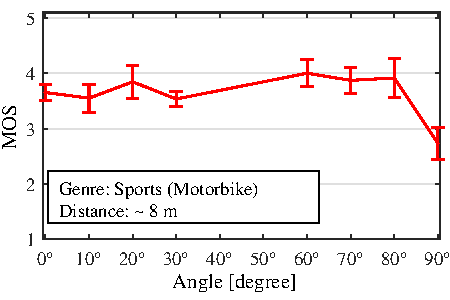
\includegraphics{./gfx/400_UGV_Quality/Angle_Sports.pdf}}
\subfloat[Music]{
	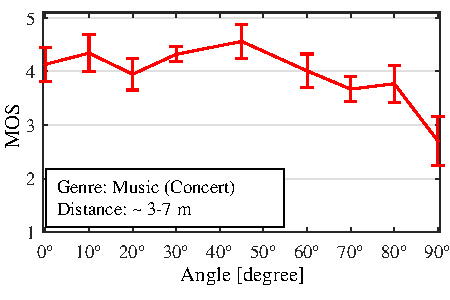
\includegraphics{./gfx/400_UGV_Quality/Angle_Music.pdf}
	}
\caption[Perceived quality from different recording angles]{Perceived quality from different recording angles at a similar recording distance.}
\label{fig:440_Angle_Sports}
\end{figure}
 Similar results were found for all genres, indicating that the recording angle does not significantly increase or decrease the perceived quality.
\section{Validation with Lab Study}
\label{sec:430_correlation}
As mentioned, a lab experiment was set up to determine if the proposed models are also valid in controlled environments.
\subsection{Recording Quality}
We want to determine the validity of the proposed, crowdsourced models with results from controlled experiment setups.
We compare the proposed quality models with results from a lab experiment for the video sequences "CrowdRun" in the genre "sports" and "DanceKiss" in genre "show".
A metric to describe the correlation between the two experiments is the Pearson correlation coefficient. 
\begin{figure}[htb]
	\centering
	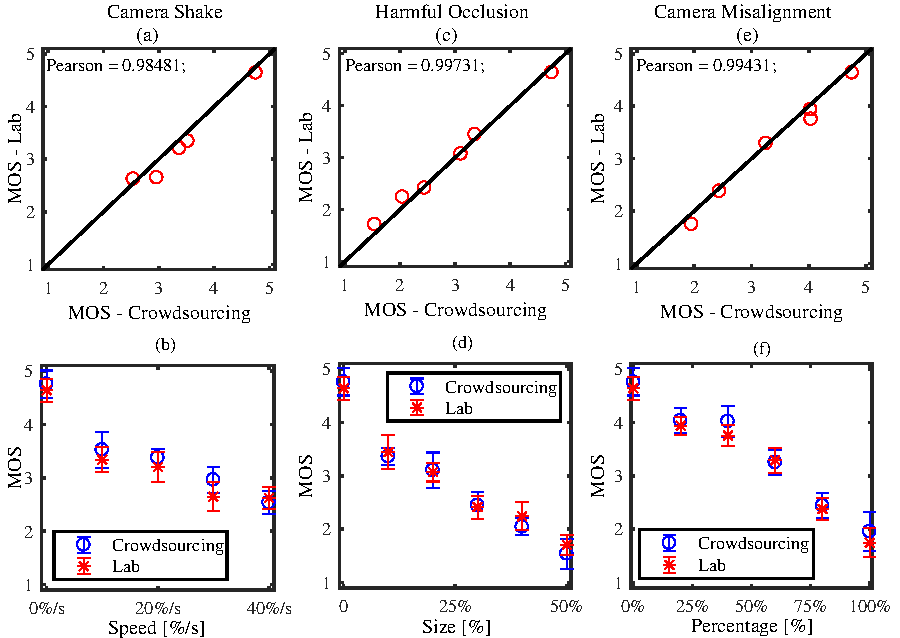
\includegraphics{gfx/400_UGV_Quality/correlation.pdf}
	\caption[Correlation of crowdourcing and lab experiments for recording degradations]{Correlation: Pearson coefficient and Confidence intervals (95\%) of MOS for the video sequence "CrowdRun". Correlation and overlap of MOS between lab and crowdsourcing experiments for Camera shakes (a)-(b), Harmful occlusions (c)-(d) and Camera Misalignment (e)-(f)}
	\label{fig:430_correlation}
\end{figure}
The Pearson's coefficient calculates how much values scatter around a linear trend.
A function is derived in which the \ac{MOS} determined in the crowdsourcing experiment describes the x-values and the lab experiment results the y-values of a linear function.
The \ac{MOS} of the lab and the crowdsourcing experiments must therefore follow a linear function, when compared with each other. This linear trend is depicted in Figure~\ref{fig:430_correlation} (a,c,e).
From the results gathered for the video "CrowdRun" a linear trend can be derived.
Furthermore, a high correlation is shown for all sequences, as values above 0.961 indicate no significant difference between the results of the crowdsourcing and the lab experiments. 

From Figure~\ref{fig:430_correlation} (b,d,f) it can be concluded that the crowdsourcing evaluation shows a big overlap with the conducted lab experiments (video sequence: "CrowdRun"), and thus our results describe the relation between the degradations and video quality in a valid manner.
\subsection{Recording Position}
Also, the models derived for assessing the perceived quality in relation to the recording distance are validated with a lab experiment.
The quality models from the genres "music", "scenery" and "show" are compared with the results from the lab experiments.
We validate only the impact of the recording distance in both the lab and crowdsourcing experiments.
Again, Pearson's coefficient is used for describing, if a linear correlation exists between the lab and crowdsourced experiments.

Especially for the genres "show" and "scenery" a high Pearson correlation of above 0.9854 and 0.937 is shown.
The "music" sequences show slightly differing results, especially for the reduced quality for increasing distances.
As a consequence, the correlation for the genre music drops to 0.7137.
In comparison to the crowdsourced tests, increasing distances are perceived to degrade the quality more. 
Even with a minimum correlation of 0.7137, it can be concluded that the retrieved quality models can be validated in both lab and crowdsourced experiments.